% Figure from MATH 591 notes, section 40. Compile with the notes preamble.
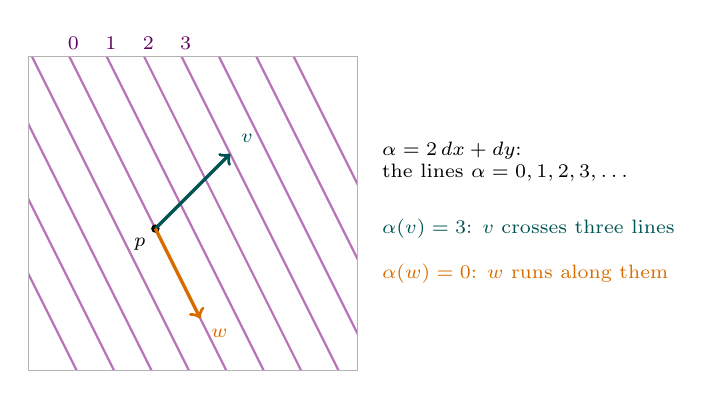
\begin{tikzpicture}[scale=0.95]
\begin{scope}
\clip (-1.7,-1.9) rectangle (2.7,2.3);
\foreach \c in {-4,...,6} \draw[violet!55, thick] ({(\c+2)/2},-2) -- ({(\c-2.4)/2},2.4);
\end{scope}
\draw[gray!60] (-1.7,-1.9) rectangle (2.7,2.3);
\foreach \c in {0,1,2,3} \node[violet!75!black, font=\scriptsize] at ({(\c-2.45)/2+0.13},2.48) {$\c$};
\fill (0,0) circle (1.6pt) node[below left, font=\scriptsize] {$p$};
\draw[->, very thick, teal!65!black] (0,0) -- (1,1) node[above right, font=\scriptsize] {$v$};
\draw[->, very thick, orange!85!black] (0,0) -- (0.6,-1.2) node[below right, font=\scriptsize] {$w$};
\node[font=\scriptsize, align=left, anchor=west] at (2.9,0.9) {$\alpha = 2\,dx + dy$:\\ the lines $\alpha = 0, 1, 2, 3, \ldots$};
\node[font=\scriptsize, align=left, anchor=west, teal!65!black] at (2.9,0.0) {$\alpha(v) = 3$: $v$ crosses three lines};
\node[font=\scriptsize, align=left, anchor=west, orange!85!black] at (2.9,-0.6) {$\alpha(w) = 0$: $w$ runs along them};
\end{tikzpicture}
